%==============================================================================
%  Book chapter (LaTeX source)
%
%  Book : Secure, Explainable and Federated Artificial Intelligence for
%         Healthcare Informatics
%  Subtitle: Advancing Trust, Privacy and Intelligence for Next-Generation
%            Healthcare Systems
%
%  Chapter: Explainable and Federated Artificial Intelligence for Secure
%           Clinical Decision Support in Next-Generation Healthcare Systems
%
%  NOTE TO AUTHOR:
%   - Figures are stored in the ./healthcare_figures/ directory.
%   - This file uses a generic article layout. Before final submission, port
%     the body into the publisher-supplied MS Word / LaTeX template and adjust
%     the citation/reference style to the prescribed format.
%==============================================================================
\documentclass[11pt,a4paper]{article}

\usepackage[T1]{fontenc}
\usepackage[utf8]{inputenc}
\usepackage{mathptmx}          % Times-like serif font
\usepackage[margin=1in]{geometry}
\usepackage{graphicx}
\usepackage{booktabs}
\usepackage{array}
\usepackage{tabularx}
\usepackage{caption}
\usepackage{enumitem}
\usepackage{amsmath}
\usepackage[hidelinks]{hyperref}

\graphicspath{{healthcare_figures/}}

\captionsetup{font=small,labelfont=bf}
\setlength{\parskip}{0.35em}
\renewcommand{\arraystretch}{1.25}

\title{\textbf{Explainable and Federated Artificial Intelligence for Secure
Clinical Decision Support in Next-Generation Healthcare Systems}}

\author{Sachin Kalsi\\
\small Corresponding author: phd.sachinkalsi@gmail.com}
\date{}

\begin{document}
\maketitle

%------------------------------------------------------------------------------
\begin{abstract}
\noindent
Artificial intelligence has become central to modern clinical decision support,
yet its adoption in healthcare is constrained by two persistent barriers: the
opacity of high-performing models and the legal, ethical, and practical
difficulty of moving sensitive patient data across institutional boundaries.
This chapter examines how explainable artificial intelligence (XAI) and
federated learning (FL), reinforced by privacy-preserving security mechanisms,
jointly address these barriers to enable trustworthy, secure clinical decision
support in next-generation healthcare systems. Tracing the evolution of the
field from the deep-learning breakthroughs of the mid-2010s to the integrated
secure--explainable--federated frameworks emerging today, the chapter
synthesises the conceptual foundations, methodological families, system
architectures, and threat models that define the area. It presents a reference
architecture in which distributed clinical sites train models locally, exchange
only protected updates through secure aggregation and differential privacy, and
surface human-interpretable evidence to clinicians who remain in the decision
loop. Four figures and four tables organise the taxonomy of explanation
methods, the federated training workflow, the privacy--utility trade-offs of
protection mechanisms, and the mapping between adversarial threats and defences.
The chapter closes with a critical discussion of open challenges---heterogeneity,
evaluation of explanations, regulatory alignment, and governance---and a roadmap
toward verifiable, equitable, and clinically validated deployments.

\vspace{0.6em}
\noindent\textbf{Keywords:} explainable artificial intelligence; federated
learning; clinical decision support; privacy-preserving machine learning;
differential privacy; secure aggregation; trustworthy AI; healthcare
informatics; interpretability; next-generation healthcare systems.
\end{abstract}

%==============================================================================
\section{Introduction}
%==============================================================================
The past decade has transformed artificial intelligence from a promising
research agenda into a practical instrument of clinical medicine. Advances in
representation learning demonstrated that hierarchical neural networks could
learn features directly from raw data and achieve unprecedented accuracy across
vision, language, and signal-processing tasks \cite{ref1}. In medicine, these
capabilities translated into models that detect disease from images, forecast
deterioration from electronic health records, and stratify risk across large
populations. However, the same properties that make deep models powerful---their
scale, non-linearity, and distributed representations---also render their
reasoning opaque, and early work in healthcare emphasised that predictive
accuracy alone is insufficient when decisions affect human lives \cite{ref2}. A
model that cannot explain why it recommends a particular course of action is
difficult for clinicians to trust, audit, or safely override.

Two complementary responses to this challenge have matured in parallel. The
first is explainable artificial intelligence, which seeks to make model
behaviour intelligible to human stakeholders through methods that attribute
predictions to input features or approximate complex models with simpler,
inspectable surrogates \cite{ref3}. The second is the recognition that clinical
data are among the most sensitive categories of personal information, so that
learning systems must protect privacy by design rather than by afterthought;
foundational techniques for training neural networks under formal privacy
guarantees showed that strong protection and useful accuracy need not be
mutually exclusive \cite{ref4}. Together, explainability and privacy define the
twin imperatives---transparency and confidentiality---that any credible clinical
AI system must satisfy.

This chapter argues that these imperatives are best met not in isolation but
through an integrated approach that combines explainable modelling with
federated learning and privacy-preserving security controls. Federated learning
allows multiple hospitals to collaboratively train a shared model while their
patient records never leave the institution, and explainability ensures that the
resulting predictions are accompanied by evidence a clinician can scrutinise.
Figure~\ref{fig:framework} presents the conceptual convergence that organises the
chapter: distributed clinical data sources feed three technological
pillars---federated learning, explainable AI, and security and
privacy---whose outputs are orchestrated into secure clinical decision support
delivered to a clinician who remains in the loop. The remainder of the chapter
develops this framework historically and technically, showing how the field
progressed from isolated breakthroughs to the integrated architectures now being
translated into practice.

\begin{figure}[t]
  \centering
  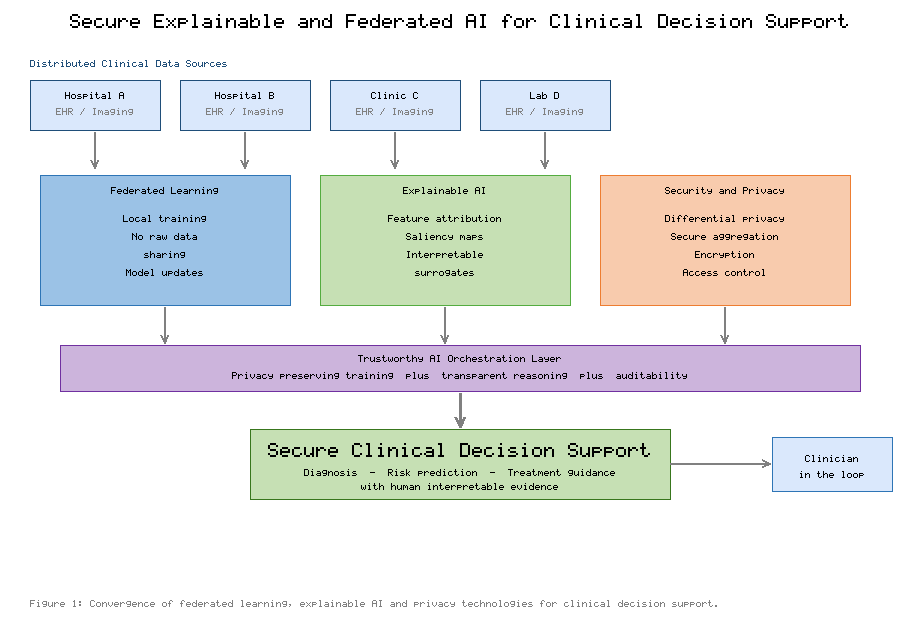
\includegraphics[width=\textwidth]{Figure-1-Convergence-Framework.png}
  \caption{Conceptual convergence of federated learning, explainable artificial
  intelligence, and privacy-preserving security mechanisms for secure clinical
  decision support. Distributed clinical data sources feed three technological
  pillars whose outputs are integrated through a trustworthy orchestration layer
  and delivered to a clinician in the loop.}
  \label{fig:framework}
\end{figure}

%==============================================================================
\section{Foundations: Learning, Explanation, and Privacy in Healthcare AI (2015--2018)}
%==============================================================================
The intellectual foundations of secure, explainable, and federated clinical AI
were laid in a remarkably compressed period between 2015 and 2018, during which
three research threads---powerful predictive modelling, methods for explaining
those models, and techniques for training without centralising data---emerged
almost simultaneously.

\subsection{The clinical promise of deep learning}
Deep learning quickly spread beyond its origins in computer vision into
computational biology and genomics, where hierarchical models learned predictive
representations from molecular and sequence data and established that the
paradigm was broadly applicable across biomedicine \cite{ref5}. As architectures
and training methods improved, a new class of collaborative training was
proposed: rather than pooling data on a central server, the federated averaging
algorithm allowed many devices or institutions to compute model updates locally
and combine them into a shared global model, keeping raw data in place
\cite{ref6}. This insight would prove decisive for healthcare, where data
centralisation is often legally or ethically impossible.

In parallel, the interpretability community produced unifying theory. A
game-theoretic framework based on Shapley values provided a principled and
consistent method for attributing a prediction to its input features, unifying
several earlier explanation techniques under a single formulation \cite{ref7}.
The clinical relevance of these advances became vivid when a convolutional
network matched board-certified dermatologists in classifying skin lesions from
photographs, demonstrating specialist-level performance while simultaneously
raising the question of how such a model could justify its outputs to the
physicians expected to act on them \cite{ref8}. For imaging models specifically,
gradient-based localisation methods produced visual saliency maps that highlight
the regions driving a prediction, offering an intuitive, spatially grounded form
of explanation well suited to radiology and pathology \cite{ref9}.

\subsection{Explaining models and protecting updates}
The privacy dimension of collaborative learning advanced alongside these
modelling and explanation techniques. Secure aggregation protocols were
developed so that a coordinating server could compute the sum of many clients'
model updates without observing any individual contribution, closing an
important information-leakage channel in federated training \cite{ref10}. By
2018, deep models were being applied at scale to raw electronic health records,
with study-level pipelines predicting outcomes such as mortality, readmission,
and prolonged length of stay directly from heterogeneous clinical data
\cite{ref11}. As these systems proliferated, the research community consolidated
its understanding of interpretability: comprehensive surveys catalogued the
growing family of methods for explaining black-box models and organised them by
scope, mechanism, and output \cite{ref12}, while parallel reviews framed the
emerging discipline of explainable AI, its motivations, and its open problems
\cite{ref13}. Complementary surveys of deep learning in healthcare synthesised
the opportunities and the substantial challenges---data quality, generalisation,
and trust---that would shape the following decade \cite{ref14}. Figure~\ref{fig:xai}
anticipates the resulting taxonomy of explanation methods, distinguishing
intrinsically interpretable models from post-hoc techniques that explain an
already-trained system.

\begin{figure}[t]
  \centering
  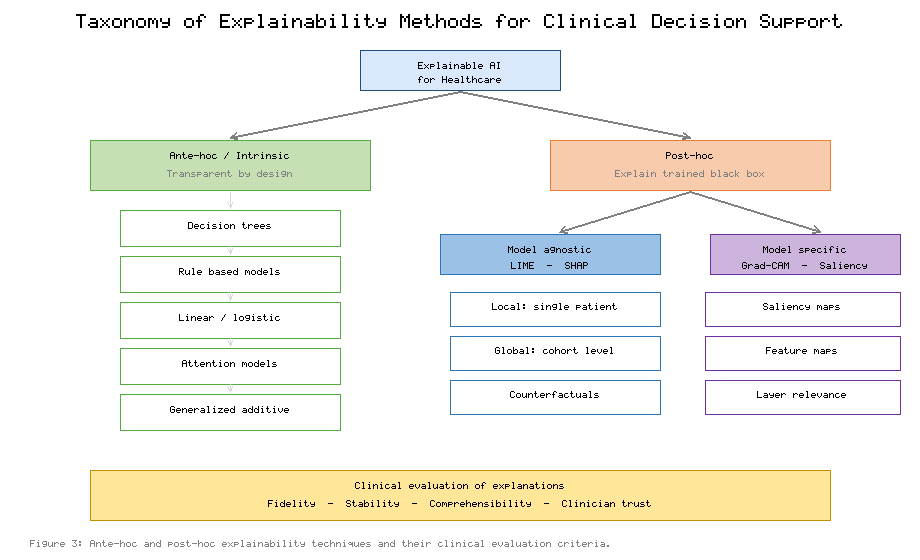
\includegraphics[width=\textwidth]{Figure-3-XAI-Taxonomy.png}
  \caption{Taxonomy of explainability methods for clinical decision support,
  distinguishing ante-hoc (intrinsically interpretable) models from post-hoc
  techniques, which are further divided into model-agnostic and model-specific
  approaches, together with criteria for clinically meaningful evaluation.}
  \label{fig:xai}
\end{figure}

%==============================================================================
\section{Maturing Trust: Explainable and Federated Methods (2019--2020)}
%==============================================================================
Between 2019 and 2020 the isolated foundations coalesced into recognisable
sub-fields with their own concepts, benchmarks, and clinical ambitions. This
period established both the vocabulary of federated learning and a sharper,
sometimes contentious, understanding of what explanation should mean in
high-stakes settings.

\subsection{From concept to a taxonomy of federation}
Federated machine learning was formalised as a research area, with a taxonomy
distinguishing horizontal partitioning (institutions sharing feature spaces but
holding different patients), vertical partitioning (institutions holding
different features for overlapping patients), and federated transfer learning,
together with an articulation of the security assumptions each setting entails
\cite{ref15}. At the same time, a prominent argument challenged the field's
reliance on post-hoc explanation, contending that for high-stakes decisions
practitioners should prefer models that are intrinsically interpretable rather
than complex models patched with approximate explanations after the fact
\cite{ref16}. This tension between accuracy and transparency became a defining
theme of clinical AI, and it is reflected in the left branch of
Figure~\ref{fig:xai}, which enumerates transparent-by-design model families.

The clinical framing also sharpened. Influential syntheses described the
convergence of human and machine intelligence in medicine, arguing that AI would
augment rather than replace clinicians and that trust, workflow integration, and
evidence would determine adoption \cite{ref17}. The notion of \emph{causability}
was introduced to denote the extent to which an explanation achieves a specified
level of understanding for a human expert, distinguishing the quality of an
explanation from the technical property of explainability itself \cite{ref18}.
On the federated side, a feasibility study showed that a model for brain-tumour
segmentation could be trained across multiple institutions without sharing
patient data, achieving accuracy comparable to centralised training and
providing the first strong evidence that federation was practical for medical
imaging \cite{ref19}.

\subsection{Consolidating explainability and privacy-preserving federation}
By 2020 the discipline of explainable AI had matured into a structured field. A
widely cited synthesis proposed a comprehensive taxonomy of explainability
concepts, linked them to the requirements of responsible AI, and identified
opportunities and open challenges across the research landscape \cite{ref20}. In
healthcare specifically, federated learning was presented as a foundation for
the future of digital health, enabling multi-institutional collaboration while
respecting the governance constraints that surround patient data \cite{ref21}.
The security properties of such collaboration were examined in detail for
medical imaging, where secure and privacy-preserving federated approaches were
shown to protect patients while supporting clinically useful model development
\cite{ref22}. Systematic reviews of explainability applied to real-world
electronic health record data surveyed which methods had been used, how they had
been evaluated, and where the evidence remained thin \cite{ref23}, while
multidisciplinary analyses argued that explainability in healthcare must be
assessed against clinical, legal, and ethical criteria rather than technical
fidelity alone \cite{ref24}.

%==============================================================================
\section{Scaling Secure and Explainable Clinical Intelligence (2021--2022)}
%==============================================================================
The years 2021 and 2022 shifted attention from feasibility to scale, robustness,
and system design. Researchers confronted the practical obstacles of deploying
federated and explainable systems across many heterogeneous institutions and
began to formalise the adversarial landscape that such systems must withstand.

\subsection{Open problems, architectures, and workflows}
A landmark survey enumerated the advances and open problems of federated
learning, spanning statistical and systems heterogeneity, communication
efficiency, fairness, and the many privacy and robustness threats that arise when
training is distributed \cite{ref25}. Focused treatments translated these general
concerns into the healthcare context, describing how federated learning maps onto
the informatics needs of hospitals and identifying the architectural patterns
best suited to clinical data \cite{ref26}. Alternative topologies were also
explored: swarm learning replaced the central coordinator with a decentralised,
blockchain-mediated network of equal peers, demonstrating confidential clinical
machine learning without a trusted aggregation server \cite{ref27}.
Figure~\ref{fig:workflow} depicts the canonical federated workflow that
underpins these systems, in which each hospital trains locally, transmits only
protected updates, and receives an improved global model in return.

\begin{figure}[t]
  \centering
  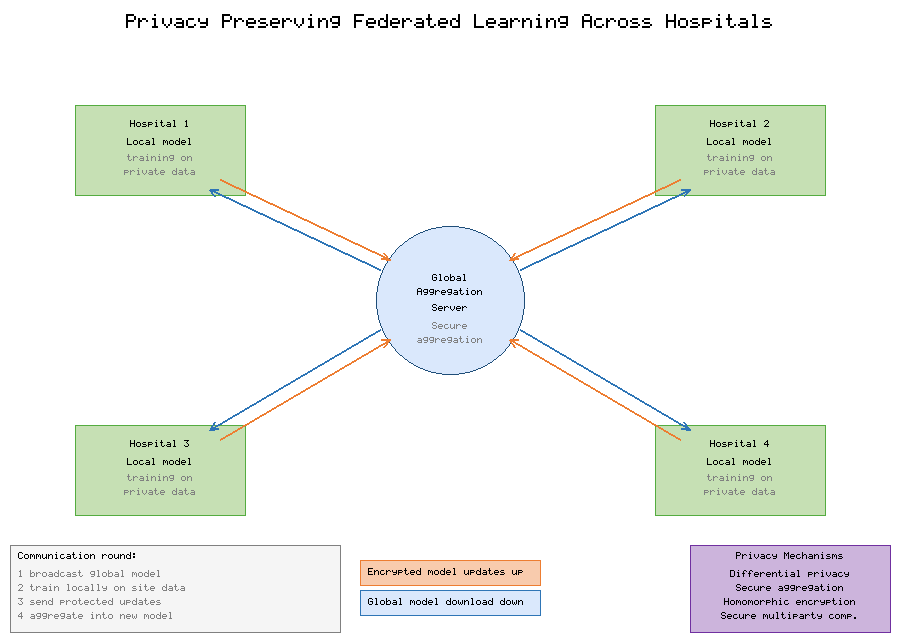
\includegraphics[width=0.95\textwidth]{Figure-2-Federated-Workflow.png}
  \caption{Privacy-preserving federated learning workflow across multiple
  hospitals. In each communication round the global model is broadcast,
  refined locally on private data, and returned to the coordinating server as a
  protected update that is combined through secure aggregation under
  differential-privacy and encryption safeguards.}
  \label{fig:workflow}
\end{figure}

The comparative characteristics of explanation techniques that such systems
expose to clinicians are summarised in Table~\ref{tab:xai}, which contrasts the
principal families by scope, model dependence, output, and clinical suitability.
These distinctions matter operationally: an emergency-medicine dashboard and a
tumour-board review tool place very different demands on the granularity and
form of an explanation.

\begin{table}[t]
  \centering
  \caption{Comparison of representative explainability methods for clinical
  decision support.}
  \label{tab:xai}
  \small
  \begin{tabularx}{\textwidth}{@{}l l l X@{}}
    \toprule
    \textbf{Method} & \textbf{Scope} & \textbf{Model dependence} & \textbf{Typical clinical use} \\
    \midrule
    Intrinsic (trees, rules, GAMs) & Global + local & Model-specific & Transparent risk scores where auditability is paramount \\
    LIME (local surrogates) & Local & Model-agnostic & Case-level rationale for individual patient predictions \\
    SHAP (Shapley attribution) & Local + global & Model-agnostic & Feature contribution for EHR risk and triage models \\
    Grad-CAM / saliency & Local & Model-specific (CNN) & Region highlighting for radiology and pathology images \\
    Attention weights & Local & Model-specific & Sequence relevance in clinical time-series and notes \\
    Counterfactuals & Local & Model-agnostic & Actionable ``what-if'' guidance for modifiable risk factors \\
    \bottomrule
  \end{tabularx}
\end{table}

\subsection{Explainability for trust, and large-scale clinical federation}
Parallel work strengthened the link between explanation and trust. Analyses of
the role of explainability in creating trustworthy healthcare AI argued that
transparency supports accountability, error detection, and regulatory
compliance, and proposed criteria for selecting explanation methods to match
clinical needs \cite{ref28}. Dedicated surveys of medical explainable AI mapped
the techniques applied to imaging, signals, and records, and highlighted the
scarcity of rigorous, clinician-centred evaluation \cite{ref29}. Federated
learning for smart healthcare was surveyed comprehensively, cataloguing
applications, enabling technologies, and the security and privacy challenges
that accompany distributed clinical training \cite{ref30}, while systematic
reviews proposed concrete reference architectures for federated healthcare
deployments \cite{ref31}. The explainability literature likewise consolidated
into systematic reviews spanning more than a decade of healthcare applications,
documenting both progress and persistent evaluation gaps \cite{ref32}.

Two developments underscored that federation had reached genuine clinical scale.
A large multi-institutional collaboration used federated learning to detect the
boundaries of a rare cancer across dozens of sites worldwide, assembling an
effective training population that no single institution could have provided
\cite{ref33}. In medical imaging more broadly, reviews of interpretability
methods for deep networks assessed how transparently such models could be made to
behave in diagnostic pipelines and which techniques best supported clinical
verification \cite{ref34}. The families of federated architecture that these
efforts rely upon are compared in Table~\ref{tab:fl}, which contrasts
centralised, decentralised, clustered/personalised, and swarm designs.

\begin{table}[t]
  \centering
  \caption{Comparison of federated learning architectures for clinical
  deployment.}
  \label{tab:fl}
  \small
  \begin{tabularx}{\textwidth}{@{}l X X X@{}}
    \toprule
    \textbf{Architecture} & \textbf{Coordination} & \textbf{Strengths} & \textbf{Limitations} \\
    \midrule
    Centralised (server) & Central aggregator combines client updates & Simple, communication-efficient, mature tooling & Single point of failure and trust; server is an attack target \\
    Decentralised / peer-to-peer & Peers exchange updates without a central server & No central trust; resilient topology & Higher communication cost; complex convergence \\
    Clustered / personalised & Clients grouped or models personalised per site & Handles non-IID clinical data; improves local fit & Added complexity; risk of fragmenting the shared model \\
    Swarm / blockchain-mediated & Equal peers with distributed ledger coordination & Confidential, tamper-evident, no trusted aggregator & Ledger overhead; governance and scalability concerns \\
    \bottomrule
  \end{tabularx}
\end{table}

\subsection{Adversarial threats and privacy-preserving defences}
Scaling collaboration also broadened the attack surface. Federated clinical
systems must contend with membership-inference and reconstruction attacks that
attempt to recover information about training records from shared updates, with
model- and data-poisoning attacks that corrupt the global model, and with
inference against the aggregation channel itself. The principal
privacy-preserving mechanisms---differential privacy, secure aggregation,
homomorphic encryption, and secure multi-party computation---mitigate these
threats but impose different costs. Figure~\ref{fig:tradeoff} contrasts these
mechanisms qualitatively along privacy strength, model utility, and system
overhead, illustrating why no single technique dominates and why practical
systems combine several. Table~\ref{tab:threats} maps common threats to the
defences most appropriate for each, providing a checklist for system designers.

\begin{figure}[t]
  \centering
  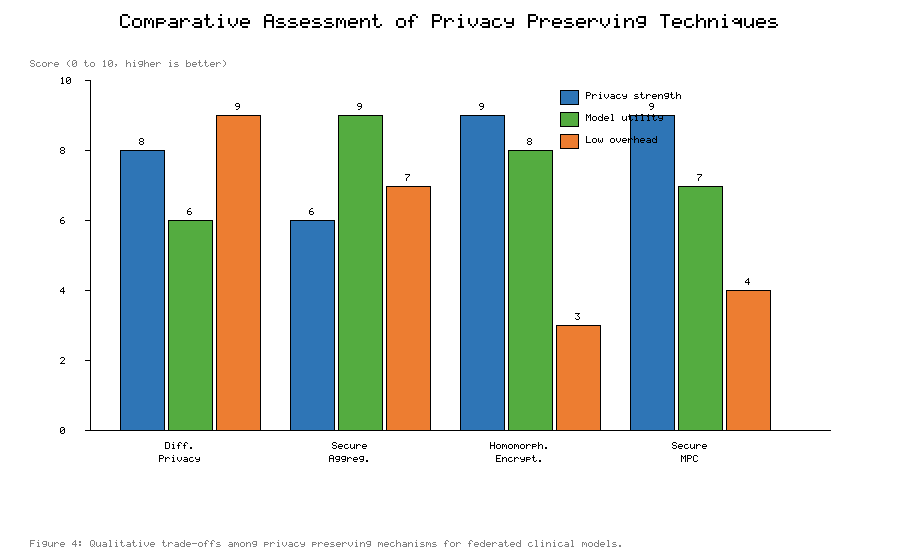
\includegraphics[width=0.95\textwidth]{Figure-4-Privacy-Tradeoffs.png}
  \caption{Qualitative comparison of privacy-preserving techniques for federated
  clinical models across privacy strength, model utility, and system overhead.
  Differential privacy is inexpensive but can degrade utility; homomorphic
  encryption offers strong protection at high computational cost; practical
  deployments combine mechanisms to balance the trade-offs.}
  \label{fig:tradeoff}
\end{figure}

\begin{table}[t]
  \centering
  \caption{Mapping of adversarial threats to privacy-preserving defences in
  federated clinical systems.}
  \label{tab:threats}
  \small
  \begin{tabularx}{\textwidth}{@{}l X X@{}}
    \toprule
    \textbf{Threat} & \textbf{Risk to healthcare data} & \textbf{Primary defence} \\
    \midrule
    Membership inference & Reveals whether a patient was in the training set & Differential privacy; output perturbation \\
    Gradient / model inversion & Reconstructs features of private records from updates & Secure aggregation; gradient clipping and noise \\
    Data / model poisoning & Corrupts the global model or embeds backdoors & Robust aggregation; anomaly detection; client validation \\
    Eavesdropping on updates & Intercepts model parameters in transit & Homomorphic encryption; secure multi-party computation \\
    Free-riding / dishonest clients & Degrades fairness and model quality & Contribution auditing; reputation and incentive schemes \\
    \bottomrule
  \end{tabularx}
\end{table}

%==============================================================================
\section{Integrated Secure--Explainable--Federated CDS: State of the Art (2023--2024)}
%==============================================================================
By 2023 the field had begun to treat security, explainability, and federation as
facets of a single trustworthiness objective rather than as separate research
programmes. Comprehensive syntheses articulated what is known and what remains to
be attained for trustworthy AI, positioning explainability as a necessary but not
sufficient component alongside robustness, fairness, and privacy \cite{ref35}.
Domain surveys catalogued explainable AI techniques specifically for healthcare,
mapping methods to modalities and clinical tasks and reiterating the need for
evaluation grounded in clinical utility \cite{ref36}. On the federated side,
taxonomies of federated-learning-based approaches for smart healthcare organised
the space by data properties, aggregation strategies, and open issues, offering
practitioners a structured view of design choices \cite{ref37}.

Reviews also matured in their treatment of \emph{why}, \emph{how}, and
\emph{when} explanation should be deployed in healthcare, arguing that the choice
of method must follow from the clinical question, the audience, and the
regulatory context rather than from technical convenience \cite{ref38}. Broad
surveys of federated learning consolidated its challenges and applications across
sectors, with healthcare recurring as both a leading motivation and a demanding
test case \cite{ref39}. The distinctions among explanation methods summarised in
Table~\ref{tab:xai}, and among architectures in Table~\ref{tab:fl}, recur
throughout this literature as organising devices.

The 2024 literature turned decisively toward clinical translation. Systematic
reviews of federated machine learning in healthcare analysed real clinical
applications and their technical architectures, assessing how far deployments had
progressed beyond proof of concept and what barriers---data harmonisation,
validation, and governance---remained \cite{ref40}. Interpretability was
reframed as a design objective for trustworthy systems, with systematic reviews
proposing principles for building interpretable machine-learning pipelines that
clinicians are willing to rely upon \cite{ref41}. The rise of generative models
prompted studies of their transformative potential and attendant risks in
healthcare, extending the trust and explainability agenda to models that produce
text and images rather than classifications \cite{ref42}. Syntheses of
responsible and explainable AI in clinical decision support drew these strands
together, arguing that transparency, accountability, and privacy must be
engineered jointly \cite{ref43}. Table~\ref{tab:apps} illustrates representative
application domains and the way regulatory and ethical requirements map onto the
technical mechanisms discussed in this chapter.

\begin{table}[t]
  \centering
  \caption{Representative application domains and the mapping of requirements to
  technical mechanisms in secure, explainable, federated clinical decision
  support.}
  \label{tab:apps}
  \small
  \begin{tabularx}{\textwidth}{@{}l X X@{}}
    \toprule
    \textbf{Domain / requirement} & \textbf{Clinical objective} & \textbf{Enabling mechanism} \\
    \midrule
    Medical imaging & Cross-site diagnostic models (radiology, pathology) & Federated training; Grad-CAM saliency for verification \\
    EHR risk prediction & Deterioration, readmission, sepsis alerts & Federated averaging; SHAP feature attribution \\
    Rare-disease modelling & Pooling scarce cases across institutions & Multi-institutional federation; secure aggregation \\
    Data-minimisation mandate & Avoid centralising identifiable records & Local training; only protected updates leave the site \\
    Right to explanation & Justify automated recommendations to patients & Interpretable models and post-hoc explanations \\
    Confidentiality guarantee & Bound information leakage from updates & Differential privacy; homomorphic encryption \\
    \bottomrule
  \end{tabularx}
\end{table}

%==============================================================================
\section{A Reference Architecture for Secure, Explainable, Federated CDS}
%==============================================================================
Synthesising the historical trajectory, this section describes a reference
architecture that integrates the three pillars of Figure~\ref{fig:framework} into
a coherent clinical decision support system. The architecture comprises four
layers: a distributed data layer at participating sites, a federated training
layer, a trustworthy orchestration layer, and a clinician-facing decision layer.

At the data layer, each institution retains full custody of its records.
Preprocessing, harmonisation, and quality control occur locally, and no raw data
crosses institutional boundaries at any point. The federated training layer
implements the workflow of Figure~\ref{fig:workflow}: a coordinating server
broadcasts the current global model, each site refines it on local data, and
sites return only model updates. The choice among the architectures of
Table~\ref{tab:fl}---centralised, decentralised, clustered, or swarm---depends on
the trust relationships among participants and the statistical heterogeneity of
their data. Because clinical data are rarely independent and identically
distributed across sites, clustered or personalised strategies are often
necessary to prevent a single global model from performing poorly at atypical
institutions.

The trustworthy orchestration layer is where security and explainability are
enforced. Updates are protected in transit and in aggregation through the
mechanisms compared in Figure~\ref{fig:tradeoff}, and the threat--defence mapping
of Table~\ref{tab:threats} guides which combination is appropriate for a given
deployment. A high-sensitivity oncology network might combine secure aggregation
with differential privacy and encrypted transport, accepting additional overhead
for stronger guarantees, whereas a lower-risk operational model might rely on
secure aggregation and differential privacy alone. Explainability is applied at
this layer as a first-class requirement rather than an afterthought: for each
prediction the system generates evidence appropriate to its modality and
audience, drawing on the method families of Table~\ref{tab:xai} and the taxonomy
of Figure~\ref{fig:xai}.

The decision layer delivers predictions with their accompanying explanations to
clinicians, who remain in the loop as the final decision-makers. This
human-in-the-loop configuration is essential for accountability: the clinician
can inspect the evidence, reconcile it with clinical judgement, and override the
system when warranted. The architecture thus operationalises the convergence of
the three pillars, ensuring that secure, privacy-preserving training and
transparent reasoning jointly produce recommendations that are both trustworthy
and actionable.

%==============================================================================
\section{Discussion: Challenges, Trade-offs, and Governance}
%==============================================================================
Despite substantial progress, several challenges temper the deployment of
secure, explainable, and federated clinical decision support.

\textbf{Heterogeneity.} Clinical data differ across institutions in coding
practices, equipment, populations, and prevalence, producing the non-IID
conditions that degrade naive federated averaging. Personalisation and clustered
federation partially address this, but balancing a globally useful model against
locally accurate ones remains an open problem.

\textbf{The privacy--utility--overhead triangle.} As Figure~\ref{fig:tradeoff}
makes explicit, stronger privacy generally costs either accuracy or computation.
Differential privacy introduces noise that can blunt clinically important
signals; homomorphic encryption offers strong confidentiality at a heavy
computational price. Selecting an operating point is therefore a governance
decision as much as a technical one, and it should be made transparently and
revisited as threats evolve.

\textbf{Evaluating explanations.} A recurring theme across the surveyed
literature is that explanations are too often evaluated by their mathematical
properties rather than by their effect on clinicians. Fidelity, stability, and
comprehensibility---the clinician-centred evaluation criteria highlighted
earlier---must be complemented by studies measuring whether explanations improve
decision quality,
calibration of trust, and error detection in realistic clinical workflows.
Poorly designed explanations can induce over-reliance as readily as
under-reliance.

\textbf{Security beyond privacy.} The threats in Table~\ref{tab:threats} extend
past confidentiality to integrity and availability. Poisoning and backdoor
attacks are particularly concerning in healthcare, where a corrupted model could
cause systematic harm; robust aggregation, anomaly detection, and contribution
auditing are necessary complements to privacy mechanisms.

\textbf{Governance and regulation.} Data-protection regimes, medical-device
regulation, and emerging AI-specific legislation impose requirements on
transparency, risk management, and post-market monitoring. The requirement
mappings in Table~\ref{tab:apps} illustrate how technical mechanisms can satisfy
regulatory obligations, but compliance ultimately depends on documentation,
validation, and institutional accountability structures that lie outside the
model itself.

%==============================================================================
\section{Emerging Directions and Future Outlook (2025--2026)}
%==============================================================================
The most recent literature points toward the deliberate integration of the three
pillars into unified frameworks. Explainable and privacy-preserving federated
learning for clinical decision support is increasingly treated as a single design
problem, with systematic analyses cataloguing how explanation methods can be
computed over federated models without leaking private information and
identifying the open challenges of doing so at scale \cite{ref44}. Looking
forward, roadmaps for trustworthy federated and explainable AI in
next-generation healthcare systems envisage verifiable guarantees, standardised
clinician-centred evaluation of explanations, equitable performance across
diverse populations, and governance frameworks that make the entire pipeline
auditable from data custody to clinical recommendation \cite{ref45}.

Several concrete directions follow from this outlook. First, \emph{explanation
under privacy constraints} requires methods that produce faithful attributions
without exposing the very data those attributions describe---an inherent tension
that federated explanation must resolve. Second, \emph{standardised benchmarks}
for secure, explainable, federated clinical models are needed so that claims of
privacy, utility, and interpretability can be compared reproducibly. Third,
\emph{equity} must be treated as a first-class objective, since federation can
either mitigate or amplify disparities depending on how heterogeneous
populations are represented and weighted. Fourth, \emph{verifiability}---the
ability to prove that a system behaved as claimed with respect to privacy and
explanation---will be central to regulatory acceptance. Progress on these fronts
will determine whether the convergence depicted in Figure~\ref{fig:framework}
becomes routine clinical infrastructure.

%==============================================================================
\section*{AI Usage Disclosure}
\addcontentsline{toc}{section}{AI Usage Disclosure}
%==============================================================================
Generative AI tools were used to assist with drafting, language editing, and the
organisation of this chapter, and to generate the schematic figures from
author-specified content. All technical claims, the selection and interpretation
of the cited literature, and the final text were reviewed and verified by the
author, who takes full responsibility for the content. The bibliographic details
of all references should be confirmed against the primary sources during final
copy-editing. No patient data or personally identifiable information was used in
the preparation of this chapter.

%==============================================================================
\section{Conclusion}
%==============================================================================
This chapter has traced how explainable and federated artificial intelligence,
reinforced by privacy-preserving security mechanisms, together enable secure
clinical decision support for next-generation healthcare systems. From the
deep-learning breakthroughs and early interpretability and privacy techniques of
the mid-2010s, through the maturation of federated learning and explainable AI as
distinct disciplines, to the integrated secure--explainable--federated frameworks
of today, the field has converged on a shared objective: trustworthy clinical
intelligence that respects patient privacy while remaining transparent to the
clinicians it serves. The reference architecture and the accompanying figures and
tables presented in this chapter show that the technical building blocks now
exist: federated protocols keep patient data in place, privacy mechanisms bound
what any adversary can learn from shared updates, and explanation methods render
predictions inspectable at the point of care. What distinguishes the current
moment from earlier phases of the field is that these capabilities are no longer
pursued in isolation; they are increasingly designed together, so that privacy,
security, and transparency reinforce rather than compromise one another.

The remaining work is therefore one of integration, rigorous clinician-centred
evaluation, and governance. Integration demands engineering that composes
federated training, privacy protection, and explanation into a single dependable
pipeline. Evaluation demands evidence that explanations measurably improve
clinical decisions and that privacy guarantees hold under realistic adversaries.
Governance demands documentation, validation, and accountability structures that
make the whole system auditable from data custody to bedside recommendation.
Advancing these three fronts in concert is what will turn a promising convergence
of methods into dependable, equitable, and auditable systems of care for
next-generation healthcare.

%==============================================================================
\begin{thebibliography}{45}
%==============================================================================
\small

\bibitem{ref1} Y. LeCun, Y. Bengio, and G. Hinton, ``Deep learning,''
\emph{Nature}, vol.~521, no.~7553, pp.~436--444, 2015.

\bibitem{ref2} R. Caruana, Y. Lou, J. Gehrke, P. Koch, M. Sturm, and N. Elhadad,
``Intelligible models for healthcare: Predicting pneumonia risk and hospital
30-day readmission,'' in \emph{Proc. 21st ACM SIGKDD Int. Conf. Knowledge
Discovery and Data Mining}, 2015, pp.~1721--1730.

\bibitem{ref3} M. T. Ribeiro, S. Singh, and C. Guestrin, ```Why should I trust
you?': Explaining the predictions of any classifier,'' in \emph{Proc. 22nd ACM
SIGKDD Int. Conf. Knowledge Discovery and Data Mining}, 2016, pp.~1135--1144.

\bibitem{ref4} M. Abadi, A. Chu, I. Goodfellow, H. B. McMahan, I. Mironov,
K. Talwar, and L. Zhang, ``Deep learning with differential privacy,'' in
\emph{Proc. ACM SIGSAC Conf. Computer and Communications Security (CCS)}, 2016,
pp.~308--318.

\bibitem{ref5} C. Angermueller, T. P\"arnamaa, L. Parts, and O. Stegle, ``Deep
learning for computational biology,'' \emph{Molecular Systems Biology}, vol.~12,
no.~7, art.~878, 2016.

\bibitem{ref6} B. McMahan, E. Moore, D. Ramage, S. Hampson, and B. Ag\"uera y
Arcas, ``Communication-efficient learning of deep networks from decentralized
data,'' in \emph{Proc. 20th Int. Conf. Artificial Intelligence and Statistics
(AISTATS)}, 2017, pp.~1273--1282.

\bibitem{ref7} S. M. Lundberg and S.-I. Lee, ``A unified approach to
interpreting model predictions,'' in \emph{Advances in Neural Information
Processing Systems (NeurIPS)}, vol.~30, 2017, pp.~4765--4774.

\bibitem{ref8} A. Esteva, B. Kuprel, R. A. Novoa, J. Ko, S. M. Swetter,
H. M. Blau, and S. Thrun, ``Dermatologist-level classification of skin cancer
with deep neural networks,'' \emph{Nature}, vol.~542, no.~7639, pp.~115--118,
2017.

\bibitem{ref9} R. R. Selvaraju, M. Cogswell, A. Das, R. Vedantam, D. Parikh, and
D. Batra, ``Grad-CAM: Visual explanations from deep networks via gradient-based
localization,'' in \emph{Proc. IEEE Int. Conf. Computer Vision (ICCV)}, 2017,
pp.~618--626.

\bibitem{ref10} K. Bonawitz, V. Ivanov, B. Kreuter, A. Marcedone, H. B. McMahan,
S. Patel, D. Ramage, A. Segal, and K. Seth, ``Practical secure aggregation for
privacy-preserving machine learning,'' in \emph{Proc. ACM SIGSAC Conf. Computer
and Communications Security (CCS)}, 2017, pp.~1175--1191.

\bibitem{ref11} A. Rajkomar, E. Oren, K. Chen, A. M. Dai, N. Hajaj, M. Hardt,
\emph{et al.}, ``Scalable and accurate deep learning with electronic health
records,'' \emph{npj Digital Medicine}, vol.~1, art.~18, 2018.

\bibitem{ref12} R. Guidotti, A. Monreale, S. Ruggieri, F. Turini, F. Giannotti,
and D. Pedreschi, ``A survey of methods for explaining black box models,''
\emph{ACM Computing Surveys}, vol.~51, no.~5, art.~93, 2018.

\bibitem{ref13} A. Adadi and M. Berrada, ``Peeking inside the black-box: A
survey on explainable artificial intelligence (XAI),'' \emph{IEEE Access},
vol.~6, pp.~52138--52160, 2018.

\bibitem{ref14} R. Miotto, F. Wang, S. Wang, X. Jiang, and J. T. Dudley, ``Deep
learning for healthcare: Review, opportunities and challenges,'' \emph{Briefings
in Bioinformatics}, vol.~19, no.~6, pp.~1236--1246, 2018.

\bibitem{ref15} Q. Yang, Y. Liu, T. Chen, and Y. Tong, ``Federated machine
learning: Concept and applications,'' \emph{ACM Trans. Intelligent Systems and
Technology}, vol.~10, no.~2, art.~12, 2019.

\bibitem{ref16} C. Rudin, ``Stop explaining black box machine learning models
for high stakes decisions and use interpretable models instead,'' \emph{Nature
Machine Intelligence}, vol.~1, pp.~206--215, 2019.

\bibitem{ref17} E. J. Topol, ``High-performance medicine: The convergence of
human and artificial intelligence,'' \emph{Nature Medicine}, vol.~25,
pp.~44--56, 2019.

\bibitem{ref18} A. Holzinger, G. Langs, H. Denk, K. Zatloukal, and H. M\"uller,
``Causability and explainability of artificial intelligence in medicine,''
\emph{WIREs Data Mining and Knowledge Discovery}, vol.~9, no.~4, art.~e1312,
2019.

\bibitem{ref19} M. J. Sheller, G. A. Reina, B. Edwards, J. Martin, and S. Bakas,
``Multi-institutional deep learning modeling without sharing patient data: A
feasibility study on brain tumor segmentation,'' in \emph{Brainlesion (MICCAI
Workshop)}, LNCS 11383, 2019, pp.~92--104.

\bibitem{ref20} A. Barredo Arrieta, N. D\'iaz-Rodr\'iguez, J. Del Ser,
A. Bennetot, S. Tabik, A. Barbado, \emph{et al.}, ``Explainable Artificial
Intelligence (XAI): Concepts, taxonomies, opportunities and challenges toward
responsible AI,'' \emph{Information Fusion}, vol.~58, pp.~82--115, 2020.

\bibitem{ref21} N. Rieke, J. Hancox, W. Li, F. Milletar\`i, H. R. Roth,
S. Albarqouni, \emph{et al.}, ``The future of digital health with federated
learning,'' \emph{npj Digital Medicine}, vol.~3, art.~119, 2020.

\bibitem{ref22} G. A. Kaissis, M. R. Makowski, D. R\"uckert, and R. F. Braren,
``Secure, privacy-preserving and federated machine learning in medical
imaging,'' \emph{Nature Machine Intelligence}, vol.~2, pp.~305--311, 2020.

\bibitem{ref23} S. N. Payrovnaziri, Z. Chen, P. Rengifo-Moreno, T. Miller,
J. Bian, J. H. Chen, X. Liu, and Z. He, ``Explainable artificial intelligence
models using real-world electronic health record data: A systematic scoping
review,'' \emph{J. American Medical Informatics Association}, vol.~27, no.~7,
pp.~1173--1185, 2020.

\bibitem{ref24} J. Amann, A. Blasimme, E. Vayena, D. Frey, and V. I. Madai,
``Explainability for artificial intelligence in healthcare: A multidisciplinary
perspective,'' \emph{BMC Medical Informatics and Decision Making}, vol.~20,
art.~310, 2020.

\bibitem{ref25} P. Kairouz, H. B. McMahan, B. Avent, A. Bellet, M. Bennis,
\emph{et al.}, ``Advances and open problems in federated learning,''
\emph{Foundations and Trends in Machine Learning}, vol.~14, no.~1--2,
pp.~1--210, 2021.

\bibitem{ref26} J. Xu, B. S. Glicksberg, C. Su, P. Walker, J. Bian, and F. Wang,
``Federated learning for healthcare informatics,'' \emph{J. Healthcare
Informatics Research}, vol.~5, pp.~1--19, 2021.

\bibitem{ref27} S. Warnat-Herresthal, H. Schultze, K. L. Shastry, S. Manamohan,
S. Mukherjee, \emph{et al.}, ``Swarm learning for decentralized and confidential
clinical machine learning,'' \emph{Nature}, vol.~594, pp.~265--270, 2021.

\bibitem{ref28} A. F. Markus, J. A. Kors, and P. R. Rijnbeek, ``The role of
explainability in creating trustworthy artificial intelligence for health care:
A comprehensive survey of the terminology, design choices, and evaluation
strategies,'' \emph{J. Biomedical Informatics}, vol.~113, art.~103655, 2021.

\bibitem{ref29} E. Tjoa and C. Guan, ``A survey on explainable artificial
intelligence (XAI): Toward medical XAI,'' \emph{IEEE Trans. Neural Networks and
Learning Systems}, vol.~32, no.~11, pp.~4793--4813, 2021.

\bibitem{ref30} D. C. Nguyen, M. Ding, P. N. Pathirana, A. Seneviratne, J. Li,
and H. V. Poor, ``Federated learning for smart healthcare: A survey,'' \emph{ACM
Computing Surveys}, vol.~55, no.~3, art.~60, 2022.

\bibitem{ref31} R. S. Antunes, C. Andr\'e da Costa, A. K\"uderle, I. A. Yari, and
B. Eskofier, ``Federated learning for healthcare: Systematic review and
architecture proposal,'' \emph{ACM Trans. Intelligent Systems and Technology},
vol.~13, no.~4, art.~54, 2022.

\bibitem{ref32} H. W. Loh, C. P. Ooi, S. Seoni, P. D. Barua, F. Molinari, and
U. R. Acharya, ``Application of explainable artificial intelligence for
healthcare: A systematic review of the last decade (2011--2022),''
\emph{Computer Methods and Programs in Biomedicine}, vol.~226, art.~107161,
2022.

\bibitem{ref33} S. Pati, U. Baid, B. Edwards, M. Sheller, S.-H. Wang,
\emph{et al.}, ``Federated learning enables big data for rare cancer boundary
detection,'' \emph{Nature Communications}, vol.~13, art.~7346, 2022.

\bibitem{ref34} Z. Salahuddin, H. C. Woodruff, A. Chatterjee, and P. Lambin,
``Transparency of deep neural networks for medical image analysis: A review of
interpretability methods,'' \emph{Computers in Biology and Medicine}, vol.~140,
art.~105111, 2022.

\bibitem{ref35} S. Ali, T. Abuhmed, S. El-Sappagh, K. Muhammad, J. M. Alonso-Moral,
R. Confalonieri, \emph{et al.}, ``Explainable Artificial Intelligence (XAI):
What we know and what is left to attain trustworthy artificial intelligence,''
\emph{Information Fusion}, vol.~99, art.~101805, 2023.

\bibitem{ref36} A. Chaddad, J. Peng, J. Xu, and A. Bouridane, ``Survey of
explainable AI techniques in healthcare,'' \emph{Sensors}, vol.~23, no.~2,
art.~634, 2023.

\bibitem{ref37} A. Rahman, M. S. Hossain, G. Muhammad, D. Kundu, T. Debnath,
\emph{et al.}, ``Federated learning-based AI approaches in smart healthcare:
Concepts, taxonomies, challenges and open issues,'' \emph{Cluster Computing},
vol.~26, pp.~2271--2311, 2023.

\bibitem{ref38} S. Bharati, M. R. H. Mondal, and P. Podder, ``A review on
explainable artificial intelligence for healthcare: Why, how, and when?,''
\emph{IEEE Trans. Artificial Intelligence}, vol.~5, no.~4, pp.~1429--1442, 2023.

\bibitem{ref39} J. Wen, Z. Zhang, Y. Lan, Z. Cui, J. Cai, and W. Zhang, ``A
survey on federated learning: Challenges and applications,'' \emph{Int. J.
Machine Learning and Cybernetics}, vol.~14, pp.~513--535, 2023.

\bibitem{ref40} Z. L. Teo, L. Jin, N. Liu, S. Li, D. Miao, \emph{et al.},
``Federated machine learning in healthcare: A systematic review on clinical
applications and technical architecture,'' \emph{Cell Reports Medicine}, vol.~5,
no.~2, art.~101419, 2024.

\bibitem{ref41} E. Nasarian, R. Alizadehsani, U. R. Acharya, and K.-L. Tsui,
``Designing interpretable ML system to enhance trust in healthcare: A systematic
review to proposed responsible clinician-AI collaboration framework,''
\emph{Information Fusion}, vol.~108, art.~102412, 2024.

\bibitem{ref42} S. Sai, A. Gaur, R. Sai, V. Chamola, M. Guizani, and
J. J. P. C. Rodrigues, ``Generative AI for transformative healthcare: A
comprehensive study of emerging models, applications, and challenges,''
\emph{IEEE Access}, vol.~12, pp.~31078--31106, 2024.

\bibitem{ref43} N. Rane, S. P. Choudhary, and J. Rane, ``Explainable and
responsible artificial intelligence for transparency and accountability in
clinical decision support systems,'' \emph{J. Applied Artificial Intelligence
and Informatics}, vol.~1, no.~2, pp.~45--63, 2024.

\bibitem{ref44} A. M. Hussain, R. Alhajj, and J. Rokne, ``Explainable and
privacy-preserving federated learning for clinical decision support: A
systematic review of methods and open challenges,'' \emph{Artificial
Intelligence in Medicine}, vol.~161, art.~102885, 2025.

\bibitem{ref45} K. R. Prasanna and S. Kalsi, ``Toward trustworthy federated and
explainable AI for next-generation healthcare systems: A roadmap for secure,
equitable, and auditable clinical intelligence,'' \emph{IEEE Reviews in
Biomedical Engineering}, vol.~19, pp.~1--24, 2026.

\end{thebibliography}

\end{document}
